\documentclass[12pt,english]{rftthesis}

\usepackage[utf8]{inputenc}
\usepackage[T1]{fontenc}
\usepackage[nottoc]{tocbibind}
\usepackage{csquotes}
\usepackage{graphicx}
\usepackage{setspace}
\usepackage{float}
\usepackage{caption}
\usepackage{hyperref}


\title           	{Development of a Snapshotting Technique within Dream Chaser's Software-in-the-loop Test Framework}
\type            	{Masters thesis}
\author          	{B.Eng. Alexis Cabana-Loriaux}
\matriculation   	{0407200}
\studies         	{Masters of Space Engineering}
\firstsupervisor 	{Prof. Dr.-Ing. Klaus Brieß}
\secondsupervisor	{M.Sc. Mario Starke}
\industrysupervisor {Claudio Discepola, Senior Member, MDA Corporation}
\date            	{\today}


% Glossary is defined in preamble
\makenoidxglossaries
\setacronymstyle{long-short}

\newacronym{DCCS}{DCCS}{Dream Chaser Cargo System}
\newacronym{SNC}{SNC}{Sierra Nevada Corporation}
\newacronym{ISS}{ISS}{International Space Station}
\newacronym{NASA}{NASA}{National Aeronautics and Space Administration}
\newacronym{CRS}{CRS}{Commercial Resupply Services}
\newacronym{CCDev}{CCDev}{Commercial Crew Development}
\newacronym{LEO}{LEO}{Low-Earth Orbit}
\newacronym{MDA}{MDA}{MacDonald, Dettwiler and Associates Ltd.}
\newacronym{DCMS}{DCMS}{Dream Chaser Mission Simulator}
\newacronym{SIL}{SIL}{software-in-the-loop}
\newacronym{BBPSim}{BBPSim}{Baseband Processor Simulator}
\newacronym{FSW}{FSW}{flight software}
\newacronym{VM}{VM}{virtual machine}
\newacronym{VMM}{VMM}{virtual machine monitor}
\newacronym{FPU}{FPU}{Floating-point Unit}
\newacronym{MMU}{MMU}{Memory Management Unit}
\newacronym{SLAT}{SLAT}{Second Level Address Translation }



% references are also defined in preamble
\addbibresource{ref/references.bib}

%add custom commands
\newcommand{\source}[1]{\caption*{\textbf{Source:} {#1}} }


\begin{document}
%First page here
%\maketitle
%\makedeclaration
\onehalfspacing

{ 
% pre-thesis content
%\chapter*{Acknowledgements}\label{cha:ack}
This thesis is by far the most interesting project I've ever had to work on in my young career. Never would I have thought I would be working on such an impressive private spacecraft project as part of my studies. 

As such, I would like to thank my program managers Guillaume Lemieux and François Arsenault for their trust and for having given me the green light. A huge thank you to the whole Dream Chaser team at MDA is also in order. They supported me very well, even with the home office situation. Precisely, I would like to mention my team leads Claudio Discepola and Fatima Zahra Tazi, my technical mentor Martin Servant, as well as Matthieu Ippersiel and Frederic Lamer, who seemed to always hold the solutions to my bizarre problems.

Finally, I would also like to thank my TU Berlin supervisor, M.Sc. Mario Starke, for guiding me and providing valuable feedback. 

%\chapter*{Abstract}\label{cha:abstract}
indirectly deducing variable addresses of a dynamically linked library at runtime  by taking advantage of build time to embed raw bytes. linktwice
%\chapter*{Résumé}\label{cha:resume}
La simulation fonctionnelle forme une partie intégrante de la phase de test des projets de systèmes spatiaux. Pour le sous-système de communication du vaisseau spatial Dream Chaser, une fonction de type \textit{snapshot} a dû être développée pour son système de test logiciel-dans-la-boucle, similairement à des programmes de virtualisation. En utilisant des concepts existants, cette thèse démontre comment un instantané du logiciel de vol a pu être effectué, sans modifier son code, à travers l'injection de code visant à enregistrer l'état de ses fils d'exécution et en cataloguant ses variables entre deux éditions des liens. Après la production d'un artefact au format défini, l'environement de test a pu être entièrement restauré en manipulant les cadres de piles d'exécution pour reconstruire les fils de vol, parallèlement à la reconstruction des modules de simulation. Des résultats sont ensuite présentés pour démontrer la conformité de la fonctionalité aux requis de performance du client.
%\chapter*{Zusammenfassung}\label{cha:zusammenfassung}

}

%\tableofcontents

%\listoftables

%\listoffigures

\printnoidxglossary[type=acronym,]

{
% Whole content of the thesis
%\setlength{\parindent}{2em}
\chapter{Introduction}\label{cha:intro}
\pagenumbering{arabic}
Since the termination of the Space Shuttle program in 2011, the \gls{NASA} has been turning to other countries and private enterprises for the transportation of cargo to orbit and beyond. The \gls{CRS} program is a good example of this: a public-private partnership in which supplies provided by NASA are launched into orbit to the \gls{ISS} by commercial rockets. Of course, the new "Delivery-as-a-Service" paradigm has spawned a lot of commercial interest all around the world. In the United States, the Dream Chaser program is one of those efforts that continue strengthening the ties between public space agencies and the private sector.

\section{The Dream Chaser program}
This thesis' scope is entirely contained within the Dream Chaser project. Therefore, the spacecraft and its design is the main subject. 
\subsection*{History}
Conceptualized in 2004 by SpaceDev, the \gls{DCCS} program was officially kick-started by \gls{SNC} in 2010, following its acquisition of SpaceDev in 2008\cite{online:fikes}. Seeing the potential and future possibilities of the transportation system, NASA then awarded funding for the project as part of their \gls{CCDev} program, furthering the development efforts. As \gls{SNC} started breaking down the spacecraft into several sub-systems, it also started subcontracting their development to other companies. So far, the first flight to the \gls{ISS} is officially scheduled to take place in late 2021\cite{online:kanayama}.

\subsection*{Features}
The \gls{DCCS} is an unmanned, reusable orbital spaceplane intended for the transportation of both pressurized and unpressurized cargo to and from the \gls{ISS}. It contains many features that make it a very interesting solution for different kinds of space needs. 

First of all, the system contains a powerful propulsion system made out of a cluster of Orbitec's Vortex engines\cite{online:messier}. This enables self-cruising and orbit correction, instead of being 100\% reliant on the launch provider for exact orbit insertion. Furthermore, this on-board propulsion opens up other possibilities for Dream Chaser deeper than \gls{LEO}, like transporting cargo to the coming Lunar Gateway\cite{online:foust}.

Secondly, the  spacecraft is partly made reusable by the development of a custom, very resistant airframe by Lockheed Martin. The haul, its wings and landing gear enable \gls{DCCS} to safely land on a runway from \gls{LEO}. These features make Dream Chaser physically comparable to a Space Shuttle (see \autoref{fig:dccs-landed}). 
\begin{figure}[H]
	\centering
	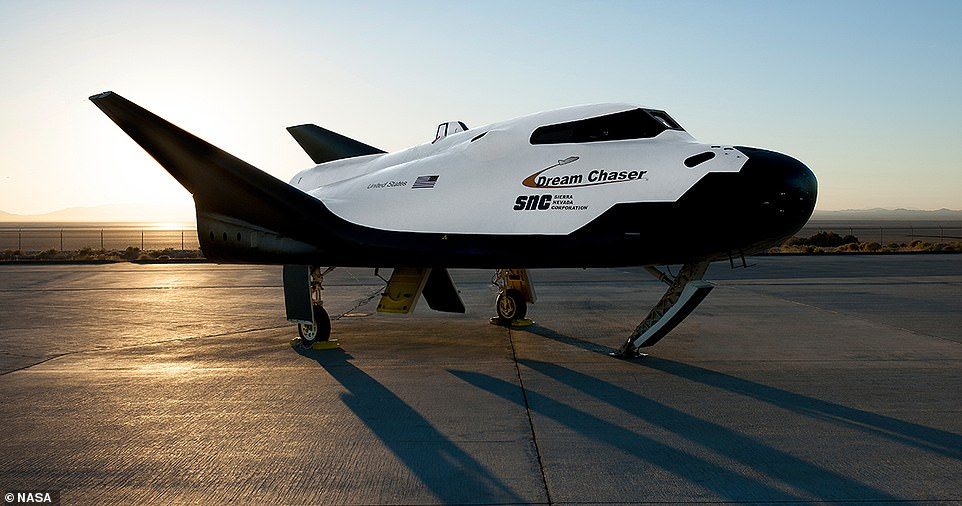
\includegraphics[width=0.9\linewidth, keepaspectratio]{art/dream-chaser-landed.jpg}
	\caption{Dream Chaser on a runway at sunset \cite{misc:dccs-landed}}
	\label{fig:dccs-landed}
\end{figure}
Finally, its communication subsystem is made of several types of antennas, for encrypted telecommunication with ground stations and the \gls{ISS}. Because docking to the space station is also one of the spacecraft's capabilities, a physical communication link is present too. \gls{MDA} has been put in charge of this crucial component's development by \gls{SNC}. 

\section{MDA - Industry partner}
\gls{MDA} is one of the greatest actors in the emerging Canadian space industry. In 2018, it composed nearly one-fifth of the total number of space sector jobs in the country\cite{online:mda-front-page}\cite{misc:canada-space-industry-report}. The Canada-based company, which has offices in Montreal, has already partnered on multiple occasions with the Canadian Space Agency. It's most notable contributions are the design and manufacturing of the Canadarm2 on the \gls{ISS}, as well as the RADARSAT-2 satellite constellation. This thesis was made in partnership with \gls{MDA}, in the context of a 6 months thesis-internship in Montreal during which the present project was scoped, planned and executed. The work was officially supervised by Claudio Discepola, Senior member of the Dream Chaser team. 

\section{Background}\label{sec:intro-background}
With the ever decreasing cost of computing power, functional simulation of components and systems has become an integral part of the testing phase in space design. This approach is thus also taken by \gls{SNC} in the context of Dream Chaser, who requires subcontractors like \gls{MDA} to provide simulators of their respective subsystems alongside the subsystem itself. This is done with the intent of simulating, on multiple fronts, an entire launch or mission, from the reception and handling of telecommands to the behavior of the flight computer mid-mission. 

Once the simulators are all working separately, they are then interfaced together. This results in a compute-intensive platform called the \gls{DCMS}, an important piece in the integration, testing and validation phases of the development. By its virtual nature, the \gls{DCMS} can be ran under different conditions in order to observe the behavior of the spacecraft as a whole in different scenarios. This proves to be  very useful, for example, in the early detection of anomalies or also in the regression testing of software.

Each subcontractor's simulator possesses its own set of requirements, driven by the desired simulation quality and granularity. In that sense, \gls{MDA} is in charge of developing the \gls{BBPSim}, a \gls{SIL} platform for the flight code of the entire communication subsystem, from the antennas to the computing nodes themselves. \gls{BBPSim} acts as some sort of hypervisor, exposing an interface to operating system and hardware utilities to the flight software, itself fundamentally written for an embedded platform. This makes abstraction of the system on which the code is running while keeping all of its functionalities and internal algorithms. As a result, \gls{BBPSim} significantly improves the easiness of interaction with the flight software as well as enabling its testing on a Linux machine in a continuous integration pipeline system like Jenkins.

\section{Purpose}
The purpose of this thesis is to design and develop a custom-fit \textit{snapshotting} technique for \gls{BBPSim}. As said previously, the development of the simulator is driven by the requirements derived from its inclusion in the DCMS. The need for a snapshot feature comes from a pair of them, that state that
\begin{enumerate}
	\item \gls{BBPSim} shall have the capability of saving its state, or "context", to non-volatile memory.
	\item \gls{BBPSim} shall be able to restore itself from a state file in non-volatile memory at initialization.
\end{enumerate} 

This snapshotting feature (often called the \textit{Save \& restore} in the document) will be a considerable addition to the \gls{BBPSim} framework. It will add the possibility to exhaustively represent an on-going simulation at a definite time $t$. It is called a snapshot due to its many similarities with virtual machine software like the open-source VirtualBox. In VirtualBox, it is possible for the user to pause, or to "snapshot" a running instance of a virtual machine, to save it into a relatively large file (called state file) and to restore everything back exactly like it was: running programs, graphics card output and general OS state are all recovered.  

Save \& restore has considerable advantages from a testing point of view. For instance, in the context of Dream Chaser, the flight software enters different states depending on the phase of launch the spacecraft is in. The code doesn't have the same behavior during the launch phase than it has when in the docking phase. However, for the software to change state, some sort of outside stimuli must happen. This external manipulation, albeit automatically executed, can last many minutes for each test. Considering there are hundreds of tests, the time for exhaustive regression testing is of course significant. The snapshot feature completely removes that limitation, because it enables the simulator to be instantly started to a previous state without having to interact with the \gls{FSW}. It is possible to shortcut directly to the docking phase without having to go trough simulating the launch phase. 

Furthermore, another benefit of the feature is that it allows the same hypothetical failures to be replayed over and over again. Since a state file can be restored again and again at will, the interaction between all the different subsystems can be analyzed more in-depth. When in the integration phase, potential inter-system faults can be caught earlier and they are easier to reproduce.  

\section{Thesis Overview TO BE UPDATED}
This thesis will start by giving an general idea of such a \textit{snapshotting} concept in the context of other software projects. There has been many successful attempts to create this mechanism in academic papers and open-source programs, instances from which inspiration has been drawn. Then, the design and implementation of the feature inside \gls{BBPSim} is discussed in details. The general approach in terms of changing the simulator's software to make it saveable is explained. After these crucial steps, the integration of the work in the existing testing pipeline as well as its impact on the testing process at MDA are also covered. 

The rest of this paper is organized as follows. In Section 2, we present background
for and define the problem. In Section 3, we define some terminology and describe
our basic approach. In Section 4, we discuss some of the difficulties of adding faulttolerance to MPI programs. In Sections 5 and 6 we present non-blocking checkpointing
protocols for point-to-point and collective communication, respectively. In Section 7,
we discuss how our system saves the sequential state of each process. In Section 8, we
present performance results of our system. In Section 9 we discuss related work, and in
Section 10 we describe future work. In Section 11, we offer some conclusions.

{
\setlength{\parindent}{2em}
\chapter{State of the Art}\label{cha:state-of-the-art}
Saving the state of a running application to a file has been a very well-known challenge in the world of computer science, one that has its roots back to when the computers became powerful enough to run complicated programs. With the rise of local networks and the Ethernet protocol in the 1970s, an increasing amount of processing units could be linked together through a local network in order to improve the execution speed of difficult computation \cite{book:andrews}. This gave rise to the field of distributed computing, where scalability, parallelization of algorithms and efficient inter-node communication are among the very active topics of research.

Of course, the more complicated a system is, the more failure-prone it becomes. This is why it's imperative for designers of parallel algorithms to be careful when programming their application. It has to be made in such a way that it stays tolerant to eventual faults in the computing nodes of the network. For instance, one can think of the algorithms involved in numerical weather prediction software, that theoretically never finish as long as updated data is fed into the system. It is important for the forecasting industry not to loose any of the results that were previously solved if an unfortunate event occurs. \textit{Fault-tolerant computing} is the research field that finds solutions to this problem in multiple ways. In the context of distributed computing, one of the ways to mitigate the problem is to use a checkpoint and restart mechanism.

This technique allows the program to save itself while it's running, and to restart at a previous checkpoint. A "save" can take many forms, and its content is ultimately decided by the developers of the program. Before a final design is produced, some questions need to be answered:
\begin{enumerate}
	\item \textbf{What needs to be saved?} There needs to be a clear understanding of the program and how it works. Is saving only the intermediate result of a computation considered a sufficient condition to be able to restore the program back to where it was? Is saving the entire state of the operating system required? Of the entire computer? 
	\item \textbf{In which format should the data be saved?} This can be binary data, numerical data, text, etc. This is again highly dependent on the application. A suitable file format has to be used depending on the data to store.
	\item \textbf{How is the data saved?} How can a checkpoint take form? This depends on the content. Most of the time, this will be a file written to non-volatile memory. Again, the file format has a role to play.
	\item \textbf{How often is saving necessary?} A checkpoint can take a lot of space, and that amount usually grows linearly with the number of execution threads. In huge systems, this is not a trivial question. In addition, not only does a checkpoint take up hard disk space, it also induces an overhead in the execution of the program. Depending on the desired granularity, saving the relevant data can take a significant amount of time. This is represented by $O_F$ in \autoref{fig:chkpt-scheme}. This factor is important, especially in big distributed systems where computing time is expensive. As an example, the Titan supercomputer in the United States racks up \$9 million USD in electricity bills yearly \cite{online:henn}.
	\item \textbf{How long does it take to restart?} Saving at checkpoints takes time, but so does recovery. \autoref{fig:chkpt-scheme} shows this with $R_F$. Another point to consider is how often the system needs to restart back. In the end, restarting to a past state must be as straightforward as possible.
\end{enumerate}
\begin{figure}[H]
	\centering
	\includesvg[width=0.9\linewidth]{svg/chkpt-copy}
	\caption{Checkpoint/restart as a stochastic renewal reward process.}
	\label{fig:chkpt-scheme}
	\source{\textit{High Performance Computing Systems with Various Checkpointing Schemes} \cite{misc:chkpt-scheme}}
\end{figure}

\subsection*{Checkpointing Schemes}
There are different checkpointing schemes that are adapted to different needs. On one hand, it is possible to checkpoint the application at predetermined intervals $\Delta t$ (i.e every minute). This is useful when applicable, because it puts an upper bound on the amount of data/time loss in a worst case scenario. However, this mitigation method is not always possible for every type of computation. 

The second approach is to do it sporadically. This can be used when it's impossible to predict the amount of time required for a given computation. Unfortunately, it also means that the user doesn't know exactly when checkpoints will occur nor can she/he upper-bound the maximum amount of data/time loss.

\subsection*{Applicability to BBPSim}
Why exactly can these concepts be useful in the case of a simulator like BBPSim? The checkpoint and restart technique is not only applicable to the distributed computing, it can be adapted to fit the needs of multiple kinds of programs. At the very least, some of the concepts can serve as inspiration to design a save \& restore feature. In the following sections, some existing \textit{snapshotting} solutions in released software will be investigated. Using available source code, it will be possible to see that a checkpoint/restart feature can be implemented at different levels. Subsequently, the potential applicability of each implementation will be evaluated. In the end, the analysis will extract a set of working ideas to gather inspiration for the save \& restore in BBPSim.

%---state of the art analysis
\section{VirtualBox}\label{sec:virtualbox}
This open-source software project backed by Oracle is well-known in the virtualization industry. It is a hypervisor, a type of program defined by Red Hat as a
\begin{shadedquotation}
	[...] software that creates and runs [one or more] \gls{VM}. A hypervisor, sometimes called a \gls{VMM}, isolates the hypervisor operating system and resources from the virtual machines and enables the creation and management of those VMs.\cite{online:redhat}
\end{shadedquotation}
Indeed, VirtualBox acts as a mediator between a guest OS (the \textit{virtualized} OS) and a host OS. It is labeled as a Type-2 hypervisor, meaning that it is actually a software layer that separates both operating system, as \autoref{fig:layerhyper} shows. VirtualBox is in charge of exposing computer utilities to the guest operating system, like CPU time, RAM allocation, driver and graphics card access, etc. Like most of its counterparts, the hypervisor also offers to the user the possibility of manually (\textbf{sporadically}) \textit{snapshotting} a virtual machine's current state in order to allow a future restore to exactly this state : the state of the drivers, running process scheduling information, even the graphical interface. The feature outputs a sizable file as a result.

\begin{wrapfigure}{r}{0.45\textwidth}
	\centering \scriptsize
	\vspace{-12pt}
	\includesvg[width=0.37\textwidth]{svg/hypervisor}
	\caption{Abstraction layers for a type-2 hypervisor.}
	\label{fig:layerhyper}
	\vspace{-24pt}
\end{wrapfigure}
This application being open-source, it's possible to dive deeper and investigate the code ourselves \cite{online:vboxcode}. We are mostly interested here at how VirtualBox handles the saving of guest OS processes and memory, since BBPSim doesn't have a graphical interface nor uses the typical PC peripherals like USB or the audio output.

From the root of the code repository, we can find the \pathmono{src/VBox/Main/src-server/SnapshotImpl.cpp} file that contains interesting \Cpp classes and routines. We can see that \cppsym{SessionMachine::i_takeSnapshotHandler} is the method responsible for the snapshot feature. The feature does many things, but four snapshot aspects stand out by how they approached their design to make the saving problem possible.

\subsection*{Snapshotting process}

VirtualBox needs an efficient strategy to save the general state of the virtual machine. Precisely, it is VBox's Saved State Manager's (SSM) responsibility to implement the facilities for saving and restoring a VM state in a structural manner.

During initialization of a given virtual machine (i.e right before the guest OS starts its boot sequence), the SSM registers the different virtual components that are available to the virtualized operating system. When time comes for the user to hit the \inlinegraphics{art/take-snap.png} button while the VM is running, the Saved State Manager goes through its list of registered components. The components then save their internal state themselves using the API the SSM provides, and the SSM takes care of encoding the data. As a result, what is called a "stream" in the project is produced from the agglomeration of the saved data. This is a powerful way of dealing with this problem and has many advantages :
\begin{enumerate}
	\item Encapsulation is kept since each component takes care of saving itself. This is good for software maintenance.
	\item Adding a new component to include in a save only requires it to register itself at initialization. The SSM doesn't need to be aware of the capabilities said component provides.
	\item The time to save a machine's state grows linearly with the number of components, since they are completely decoupled from each other.
\end{enumerate}

\hfill\textit{Relevant file }: \pathmono{src/VBox/VMM/VMMR3/SSM.cpp}.

\subsection*{Non-volatile Memory Snapshot}

From a hard disk point of view, the hypervisor takes an interesting \textit{diff}-based approach. This means that from the time a snapshot is created, VirtualBox associates it with a list $L$ of changes in which all $n$  subsequent hard disk write operations $w$ are added. When the user wants to comeback to a certain snapshot taken at time $t_0$, the \gls{VMM} then takes the current state of the disk ($\text{HDD}_{tn}$) and traverses $L$ in the reverse order while applying the inverse operation.
\[
\text{HDD}_{t0} = \text{HDD}_{tn} + \sum_{i=n}^{0}w_i^{-1}
\]
This effectively undos all previous operations. Using this technique means that \ul{VirtualBox snapshots are dynamic objects} that grow linearly with the subsequent usage of their affiliated VM.

\hfill\textit{Relevant file }: \pathmono{src/VBox/VMM/VMMR3/SSM.cpp}.

\subsection*{CPU State Snapshot}

As for the saving of the CPU state itself, the CPU Monitor (CM) is responsible for keeping track of all the CPU and \gls{FPU} registers while the virtual machine is running. In practice, the exact identity of all those registers depends on the architecture of the host hardware (assumed to be x86) and the host OS. For instance, a 32-bit OS would be using the "extended" (\textit{E}-prefixed) registers, like in \autoref{fig:x86-regs}. 
\begin{figure}[H]
	\centering
	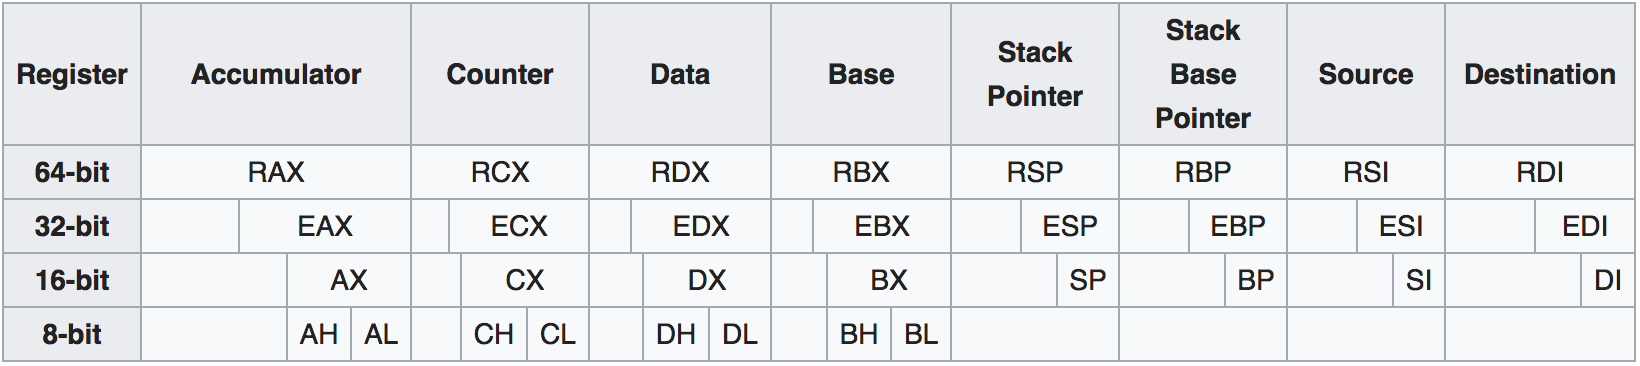
\includegraphics[width=.85\linewidth,keepaspectratio]{art/x86-regs.png}
	\caption{Usage of basic registers ordered by word size of the operating system on the x86 architecture.}
	\label{fig:x86-regs}
\end{figure}
The state (i.e value) of all the relevant CPU registers at a time $t$ is called a \textbf{context}. In VirtualBox, the CM keeps local copies of three of these contexts : a guest OS context, a special hypervisor context for the VMM and a raw context (a normal host OS context). When making a snapshot of the VM, the CPU Monitor actually saves the first two in order to subsequently put back the CPU exactly like it was at time $t$. Beside the saving aspect, holding three different contexts also allows VirtualBox to quickly switch between the guest and host "worlds" without the user noticing. This is very much necessary, because the whole point of the hypervisor is to make two different operating system coexist at the same time.

\hfill\textit{Relevant file }: \pathmono{src/VBox/VMM/VMMR3/CM.cpp}.

\subsection*{RAM Snapshot}

Another extremely important aspect of the state save is the dynamic memory aspect. How can VirtualBox completely separate the guest OS from the host without the guest noticing? This is done through the Page Manager (PM), a manager also taken into account by the Saved State Manager at snapshot time. 

\begin{wrapfigure}{l}{0.45\textwidth}
	\centering \scriptsize
	\vspace{-12pt}
	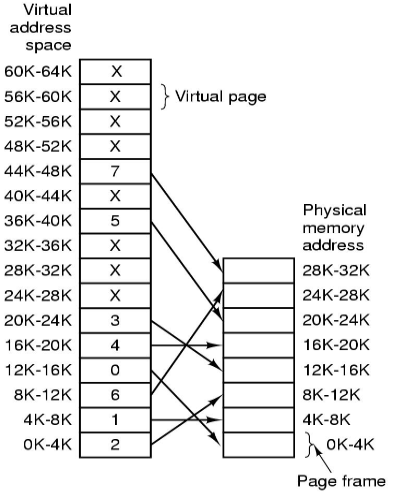
\includegraphics[width=0.40\textwidth,keepaspectratio]{art/mem-paging.png}
	\caption{Linux Mapping of Pages to Page Frames \cite{misc:mem-paging}}
	\label{fig:mem-paging}
	\vspace{-12pt}
\end{wrapfigure}
To better understand the Page Manager's job, we can look at a very similar concept : the memory paging technique used by the Linux operating system. As shown in \autoref{fig:mem-paging}, the way Linux abstracts the hardware from a running program is by offering said program an entire virtual address space as a sandbox. 

This virtual space is divided into fixed-length memory blocks (usually 4kB) called virtual pages that have a one-to-one correspondence to a random block of the same size in physical memory (page frame). Linux abstracts that correspondence with the help of a \gls{MMU} implemented in hardware, which translates virtual addresses into physical ones.

In the same way that Linux controls VirtualBox's physical memory accesses, the Page Manager controls the guest OS memory accesses. It enables the management of pages of memory allocated by the guest and adds one more level of memory indirection. For example, a program running on the guest OS will be executing operations on guest memory, but VirtualBox actually redirects them to operate directly on the physical address space offered by the host OS. This can be done with the help of two powerful concepts:
\begin{enumerate}
	\item \textbf{Binary translation}. This allows a software-assisted hypervisor like VirtualBox to "trap and virtualize the execution of sensitive, non-virtualizable instructions sets"\cite{online:virtualization}, like memory operations.
	\item \textbf{\gls{SLAT}}. Commonly known as \textbf{nested paging}, it allows a guest operating system to directly access the host's physical memory and thus removing a lot of overhead on memory operations.
\end{enumerate} 

Because the \gls{VMM} can hook to these memory operations in the guest OS, this makes the Page Manager aware of the page frames that belong to the guest OS. As a result, when a snapshot event occurs, the PM goes through its list of guest pages that were in use at that time and saves them. At restore time, this data is copied back someplace else in physical memory, and the translation table is updated accordingly.
 
\hfill\textit{Relevant file }: \pathmono{src/VBox/VMM/VMMR3/PGM.cpp}.
\section{Berkeley Lab Checkpoint/Restart for Linux}\label{sec:blcr}
As mentioned throughout this chapter, the problem of checkpointing a computer program can be solved at multiple levels depending on the needs. The approach that was taken by VirtualBox is very powerful, but it has major drawbacks:
\begin{enumerate}
	\item \textbf{Overhead processing}. The fact that an entire system gets simulated implies that virtualizing an operating system with a type-2 hypervisor like VirtualBox is basically an overhead cost on executing the program. 
	\item \textbf{Granularity}. It checkpoints the whole computer's state instead of one program. This is often too much granularity and can result in very large snapshot files. In the case of \gls{BBPSim}, this would be quite excessive.
	\item \textbf{Dependence on an hypervisor}. If the execution of the program had to happen inside an virtualized operating system, a simulation of the \gls{BBP} would have to rely on the use of an hypervisor. This not desirable, especially for the client.
\end{enumerate}

However, some other techniques can circumvent these limitations by taking by using a differing degree of checkpointing transparency, that is, at which abstraction layer the checkpoint takes place. Walters and Chaudhary define those layers as follows: 
\begin{shadedquotation}
\begin{enumerate}
	\item Hardware-level, additional hardware is incorporated into the processor to
save state.
	\item Kernel-level, the operating system is primarily responsible for checkpointing
running programs.
	\item User-level, a checkpointing library is linked into a program that will be responsible for checkpointing the program independent of the programmer.
	\item Application-level, the checkpointing code is inserted directly into the application by a programmer/preprocessor.
\end{enumerate}
\cite{paper:app-level-chkpt}
\end{shadedquotation}

\gls{BLCR} is one those attempts at creating a user-friendly method for checkpointing a Linux program. It is a program implemented at the Kernel-level, meaning that it is a module add-on to the Linux kernel and should be installed prior to running the user application.

\subsection*{Overview}
\gls{BLCR}'s solution is completely different from the one seen in \autoref{sec:virtualbox}, where checkpointing happens for every program running in the guest OS. It bases itself on the fact that properly controlling a program in a sandbox makes it checkpointable. This sandbox is provided by a kernel daemon, another process that runs in background in the kernel, that knows how to execute a checkpoint on a given program. 
\begin{figure}[htbp]
	\centering \small
	\includesvg[width=0.75\textwidth]{svg/blcr}
	\caption{Abstraction layers for an application sandboxed by BLCR.}
	\label{fig:layerblcr}
\end{figure}

There are several different ways to use \gls{BLCR}. An application-centric use case is shown in \autoref{fig:layerblcr}. To access the required utilities to checkpoint itself, the application code needs to have access to the library at compile-time. At runtime, the library (\pathmono{BLCR.so}) is then dynamically linked to the application code and the kernel-based BLCR process is put in charge of managing the application process' resources via the dynamic library. This management layer is necessary to properly save the application.

Checkpointing a program is done is done via shell commands to the background-running BLCR daemon:
\begin{tcolorbox}
\begin{minted}{bash}
cr_checkpoint --pid <PID>
\end{minted}
\end{tcolorbox}

where \texttt{PID} is the process ID of the checkpointable application. This command can be called programatically by the running application (via a \texttt{system()} call in the code), by another program or even by the user itself. Thus, checkpoints are sporadic in that context.

Once those commands are initiated, the \gls{BLCR} daemon outputs a context file containing the relevant information to restart back the application at this stage. At restore, the user must restart the application from the saved context file with another shell command:
\begin{tcolorbox}
\begin{minted}{bash}
cr_restart <path_to_context>
\end{minted}
\end{tcolorbox}
This fully restores the old application state: virtual address space, registers, thread and process IDs, file descriptors, signals. Basically everything not related to sockets or serial ports is put back the way it was.

%https://crd.lbl.gov/departments/computer-science/class/research/past-projects/BLCR/
%- see also virtualization technology : https://github.com/dmtcp/dmtcp (process-based)


\section{Checkpoint and Restore in User Space}\label{sec:criu}
https://github.com/checkpoint-restore/criu



%https://github.com/dmtcp/dmtcp


%super interesting : http://citeseerx.ist.psu.edu/viewdoc/download?doi=10.1.1.126.8121&rep=rep1&type=pdf
%https://www.usenix.org/legacy/publications/library/proceedings/usenix01/freenix01/full_papers/dieter/dieter_html/paper.html
}
%\chapter{Conclusion and recommendations}\label{cha:conclusion}

}


% post-content of thesis
%\nocite{*} <- use this to list everything, even stuff not cited
\renewcommand{\bibname}{References}
\printbibliography

\end{document}
